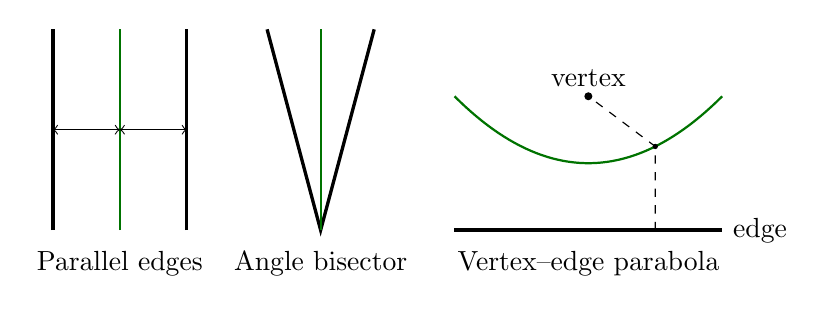
\begin{tikzpicture}[scale=.85]
\draw[very thick] (0,0)--(0,3) (2,0)--(2,3);
\draw[green!45!black,thick] (1,0)--(1,3);
\draw[<->] (0,1.5)--(1,1.5);\draw[<->] (1,1.5)--(2,1.5);
\node at (1,-.5) {Parallel edges};
\begin{scope}[shift={(4,0)}]
\draw[very thick] (-.8,3)--(0,0)--(.8,3);
\draw[green!45!black,thick] (0,0)--(0,3);
\node at (0,-.5) {Angle bisector};
\end{scope}
\begin{scope}[shift={(8,0)}]
\draw[very thick] (-2,0)--(2,0) node[right] {edge};
\fill (0,2) circle(.06) node[above] {vertex};
\draw[green!45!black,thick,domain=-2:2,samples=50] plot (\x,{1+\x*\x/4});
\fill (1,1.25) circle(.04);
\draw[dashed] (1,0)--(1,1.25)--(0,2);
\node at (0,-.5) {Vertex--edge parabola};
\end{scope}
\end{tikzpicture}
